\chapter{Memoria Descriptiva}

Hola como estan mis kines

\section{Descripción general del proyecto}

\section{Objetivos de la obra}

\section{Ubicación y área de intervención}

El proyecto se desarrolla en el edificio de la \textbf{Escuela Profesional de Enfermería}, interviniendo tres niveles específicos identificados en los planos. Cada piso tiene dimensiones aproximadas de 38.70 m de largo x 19.71 m de ancho, con un área útil aproximada de 763 m² por nivel, sumando unos 2 289 m² totales de intervención.:

\begin{itemize}
    \item \textbf{Primer Nivel (Área Administrativa y Lectura):} Incluye salas como Secretaría Docente, Decanato, Coordinación, Jefatura, Sala de Lectura, Almacén de Libros y Editorial.
    
    \item \textbf{Segundo Nivel (Área Académica):} Comprende las Aulas 201, 202, 203, 204 y ambientes de apoyo.
    
    \item \textbf{Tercer Nivel (Laboratorio y Grados):} Intervención en el Salón de Grados, Laboratorios (Ambientes 404, 405) y una sala de cómputo de alta densidad.
\end{itemize}

\section{Alcances del proyecto}

\textbf{Teoría:} Los alcances definen cuantitativamente qué se va a instalar: número de puntos de red (tomas de datos/voz), cantidad de racks o gabinetes de telecomunicaciones, y la cobertura que se pretende lograr (100\% de los ambientes, redundancia, etc.). Este apartado es la base del presupuesto y el cronograma. Se apoya en estándares como la \textbf{TIA-568} (cableado estructurado) y la \textbf{TIA-569} (espacios y trayectorias), que establecen una densidad mínima de 2 puntos por estación de trabajo y al menos 1 rack por cada 1 000 m² o por piso.

De acuerdo con el análisis de los planos proporcionados, el alcance físico incluye:

\begin{itemize}
    \item \textbf{Cantidad de puntos de red}: Se han identificado un total de \textbf{28 puntos de datos} (etiquetados como G09-Dxx) distribuidos de la siguiente manera:
    \begin{itemize}
        \item Piso 1: 7 puntos (D01 a D07) triangulos azules
        
            \begin{figure}[H]
                \centering
                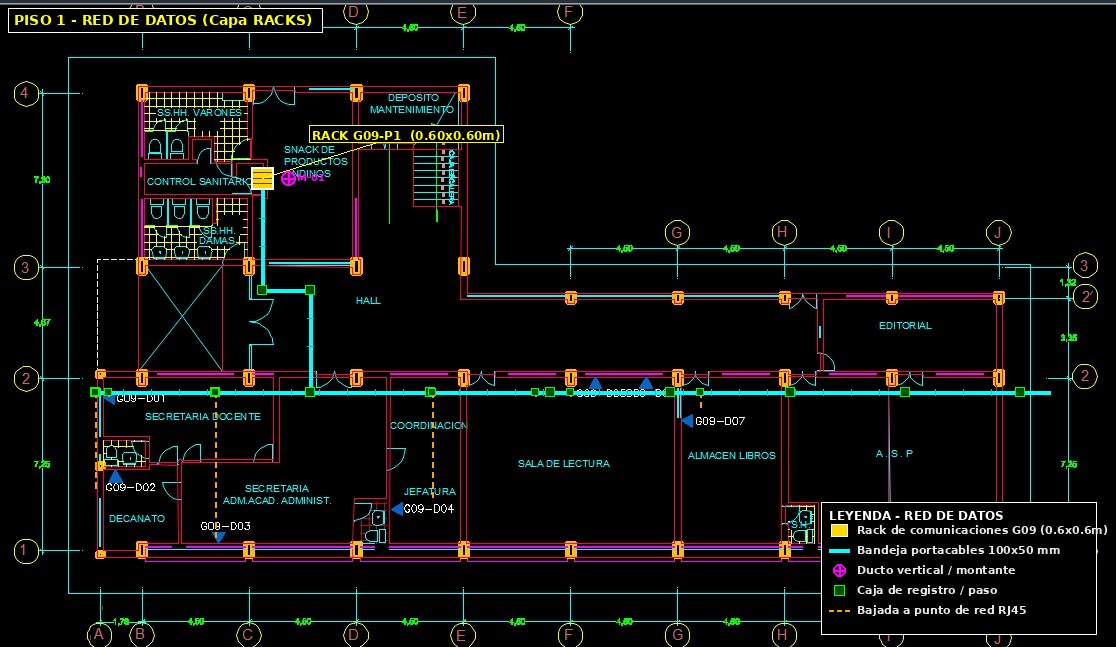
\includegraphics[width=1.0\linewidth]{figures/figuresMarco/primer_nivel.jpeg}
                \caption{}
                \label{fig:placeholder}
            \end{figure}

        \item Piso 2: 6 puntos (D08 a D13)
        
            \begin{figure}[H]
                \centering
                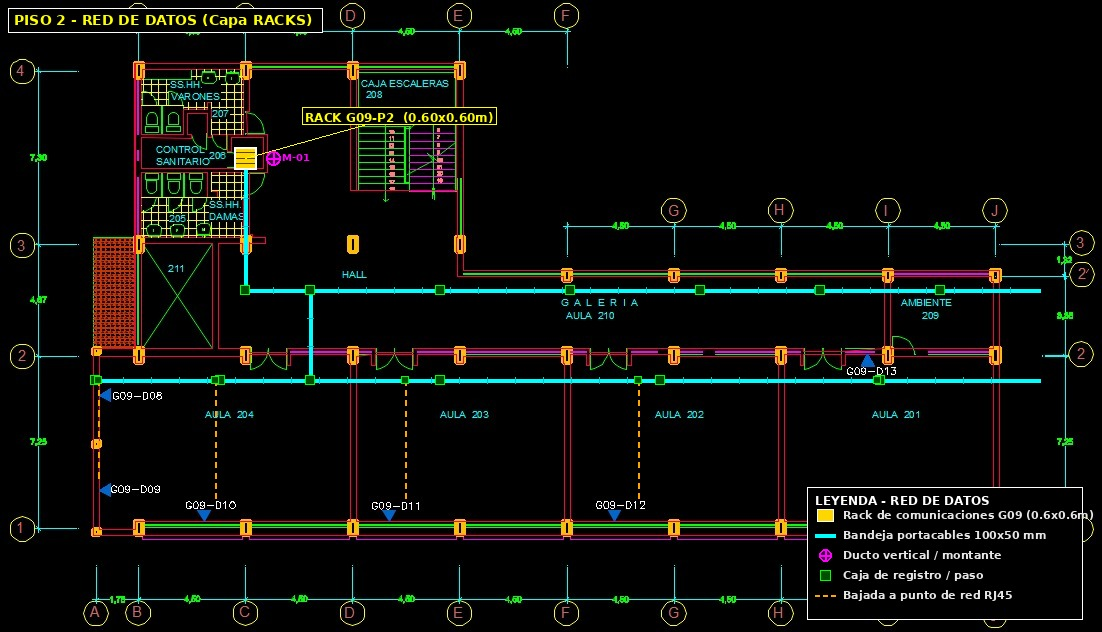
\includegraphics[width=1.0\linewidth]{figures/figuresMarco/segundo_nivel.jpeg}
                \caption{}
                \label{fig:placeholder}
            \end{figure}


        \item Piso 3: 15 puntos (D14 a D29), destacando el laboratorio con 10 puntos concentrados
        
            \begin{figure}[H]
                \centering
                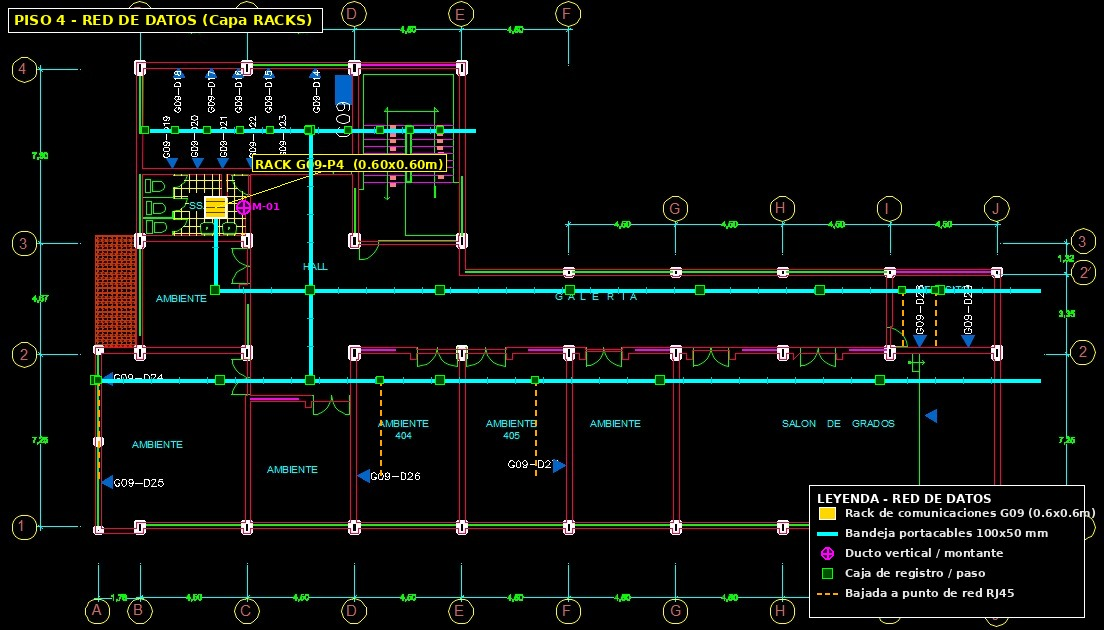
\includegraphics[width=1.0\linewidth]{figures/figuresMarco/tercer_nivel.jpeg}
                \caption{}
                \label{fig:placeholder}
            \end{figure}

    \end{itemize}
    
    \item \textbf{Racks}: Se proyecta \textbf{1 Rack Principal (MDF)} ubicado en el Tercer Nivel (identificado como el bloque azul G09), que centralizará la conexión de todo el edificio
    
    \item \textbf{Cobertura}: 100\% de las oficinas administrativas, aulas teóricas y laboratorios especializados
\end{itemize}

\section{Justificación técnica y beneficios}

\section{Normas y estándares aplicados}
